\chapter{Calendar dates}
\label{chap:calendar}

\section{Introduction}
\label{sec:cal-intro}

Any software that aims to handle dates and times must have a good
built-in calendar. Gretl offers several functions to handle date and
time information, which are documented in the \GCR{}. To facilitate
their effective use this chapter lists the various possibilities for
storing dates and times and discusses ways of converting between
variant representations.  Our main focus in this chapter is dates as
such (year, month and day) but we add some discussion of time-of-day
where relevant. A final section addresses the somewhat arcane issue
of handling historical dates on the Julian calendar.

First of all, however, it may be useful to distinguish two contexts:
\begin{itemize}
\item You have a time-series dataset in place, or a panel dataset with
  a well-defined time dimension.
\item You have no such dataset in place, or perhaps no dataset at all.
\end{itemize}

While you can work with dates in the second case, in the first case
you have extra resources.

You probably know that if you open a dataset that is in fact time
series but gretl has not immediately recognized that fact, you can
rectify matters by use of the \cmd{setobs} command, or via the menu
item \textsf{/Data/Dataset structure} in the gretl GUI. You may also
know that with a panel dataset you can impose a definite dating and
frequency in its time dimension (if appropriate)---again, via the
\cmd{setobs} command but with the \option{panel-time} option.

In what follows we state if a relevant function or accessor requires a
time-series dataset or well-defined panel-data time; otherwise you can
assume it does not carry such a requirement.

\section{Date and time representations}
\label{sec:cal-representations}

In gretl there is more than one way to encode a date such as ``May
26th, 1993''. Some are more intuitive, some less obvious from the
viewpoint of a human but easier to handle for an algorithm. The basic
representations we discuss here are:
\begin{enumerate}
\item the three-numbers approach
\item date as string
\item the ISO 8601 standard
\item the epoch day
\item Unix time (seconds)
\end{enumerate}
We first explain what these representations are, then explain how
to convert between them.

\subsection{The three-numbers approach}
\label{sec:cal-3numbers}

Since a date (without regard to intra-day detail) basically consists
of three numbers, it can obviously be encoded in precisely that way.
For example the date ``May 26th, 1993'' can be stored as
\begin{code}
  scalar y = 1993
  scalar m = 5
  scalar d = 26
\end{code}

Gretl's multiple-element objects can be used to extend this approach,
for example by using a 3-element vector for year, month and day, or a
3-column matrix for storing as many dates as desired. If you wish to
store dates as series in your dataset this approach would lead you to
use three series, possibly grouping them into a list, as in
\begin{code}
  nulldata 60
  setobs 7 2020-01-01
  series y = $obsmajor
  series m = $obsminor
  series d = $obsmicro
  list DATE = y m d
\end{code}
%$
This example above will generate daily dates for January and February
2020. Note that use of the \verb|$obsm*| accessors requires a
time-series dataset, and \dollar{obsmicro} in particular requires
daily data. See Section~\ref{sec:cal-otherfuncs} for details.

Some CSV files represent dates in this sort of broken-down format,
with various conventions on the ordering of the three components.

\subsection{Date as string}
\label{sec:cal-generic-string}

To a human being, this may seem the most natural choice.  The string
``26/6/1953'' is pretty much unambiguous. But using such a format for
machine processing can be problematic due to differing conventions
regarding the separators between day, month and year, as well as the
order in which the three pieces of information are arranged.  For
example, ``2/6/1953'' is \textit{not} unambiguous: it will
``naturally'' be read differently by Europeans and Americans. This can
be a problem with CSV files found ``in the wild'', containing
arbitrarily formatted dates. Therefore gretl provides fairly
comprehensive functionality for converting dates of this sort into
more manageable formats.

\subsection{The ISO 8601 standard}
\label{sec:cal-ISO8601}

Among other things, the ISO 8601 standard provides two representations
for a daily date: the ``basic'' representation, which uses an 8-digit
integer, and the ``extended'' representation, which uses a
10-character string.

In the basic version the first four digits represent the year, the
middle two the month and the rightmost two the day, so that for
example \texttt{20170219} indicates February 19th, 2017. The extended
representation is similar except that the date is a string in which
the items are separated by hyphens, so the same date would be
represented as ``\texttt{2017-02-19}''.

In several contexts ISO 8601 dates are privileged by gretl: the ISO
format as taken as the default and you need to supply an additional
function argument or take extra steps if the representation is
non-standard.

Using series and/or matrices to store ISO 8601 basic dates is
perfectly straightforward.

\subsection{Epoch days}
\label{sec:cal-epochday}

In gretl an ``epoch day'' is an unsigned 64-bit integer which
represents a date as the number of days since January 1, 1 AD (that
is, the first day of the Common Era), on the proleptic Gregorian
calendar.\footnote{The term ``proleptic,'' as applied to a calendar,
  indicates that it is extrapolated backwards or forwards relative to
  its period of actual historical use.} For example, 1993-05-26
corresponds to 727709.\footnote{This representation derives from the
  astronomers' ``Julian day'' which is also a count of days since a
  benchmark, namely January 1, 4713 BC, at which time certain
  astronomical cycles were aligned.}

This is the convention used by the \textsf{GLib} library, on which
gretl depends for much of its calendrical calculation. Since an epoch
day is an unsigned integer, neither \textsf{GLib} nor gretl supports
dates ``BC'', or prior to the Common Era.

This representation has several advantages. Like ISO 8601 basic, it
lends itself naturally to storing dates as series. Compared to ISO
8601, it has the disadvantage of not being readily understandable by
humans, but to compensate for that it makes it very easy to determine
the length of a range of dates.  ISO basic dates can be used for
comparison (which of two dates, on a given calendar, refers to a later
day?) but with epoch days one can carry out fully-fledged ``dates
arithmetic.''  Epoch days are always consecutive by construction, but
8-digit basic dates are consecutive only within a given
month.\footnote{In fact, they advance by 101 minus the number of days
  in the previous month at the start of each month other than
  January, and by 8870 at the start of each year.} For more on
arithmetic with epoch days see Section~\ref{sec:cal-arith}.

\subsection{Unix seconds}
\label{sec:cal-seconds}

In this representation---the cornerstone of date and time handling on
Unix-like systems---time is the number of seconds since midnight at
the start of 1970 according to Coordinated Universal Time
(UTC).\footnote{UTC is, to a first approximation, the time such that
  the Sun is at its highest point at noon over the prime meridian, the
  line of 0\textdegree{} longitude, which as a matter of historical
  contingency runs through Greenwich, England.}  This format is
therefore ideal for storing fine-grained information, including time
of day as well as date.

This representation is not transparent to humans (for example, the
number 123456789 corresponds to the start of Thursday, 29 Nov 1973)
but again it lends itself naturally to calculation. Since Unix seconds
are hard-wired to UTC a given value will correspond to different
times, and possibly different dates, if evaluated in different time
zones; we expand on this point below.

\section{Converting between representations}
\label{sec:cal-conversions}

\begin{figure}[htbp]
  \centering
  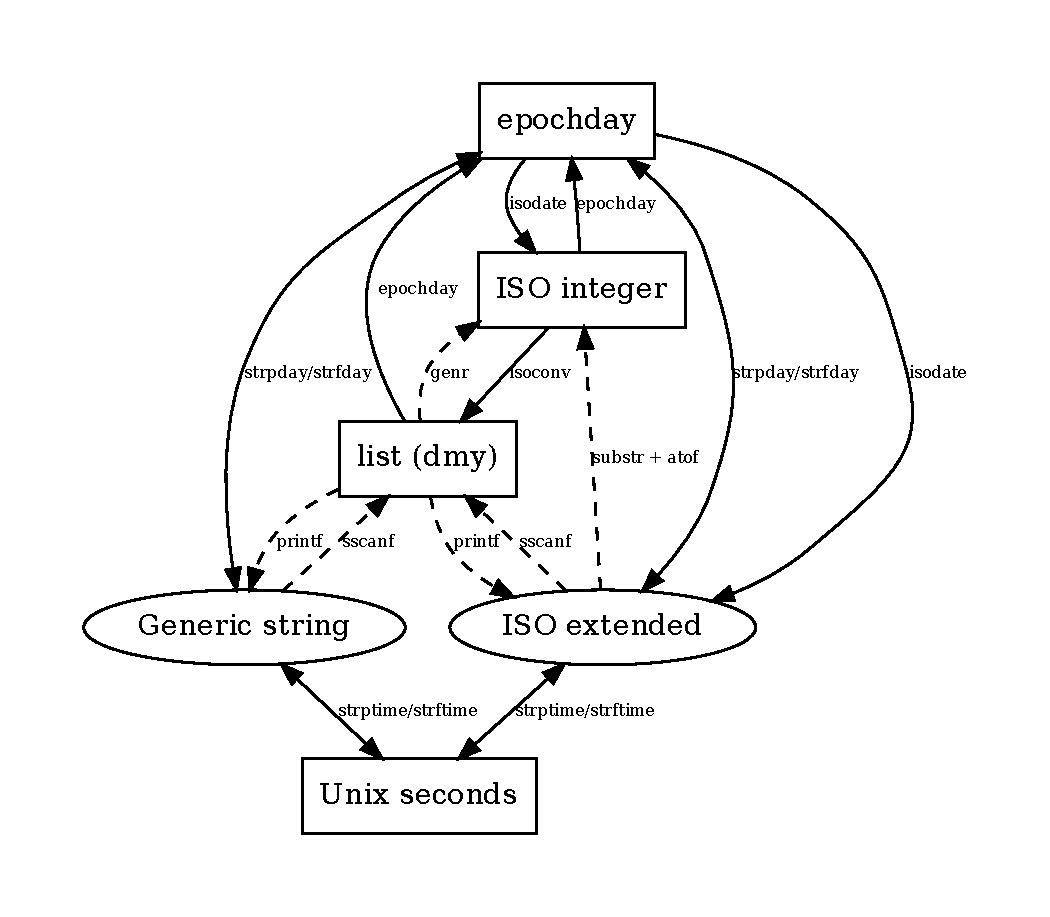
\includegraphics[scale=0.667]{figures/date-conversion}
  \caption{Conversions between different date formats}
  \label{fig:cal-conversions}
\end{figure}

To support conversion between different representations, gretl
provides several dedicated functions, although in some cases
conversion can be carried out by using general-purpose
functions. Figure \ref{fig:cal-conversions} displays a summary: solid
lines represent dedicated functions, while dashed lines indicate that
no special function is needed. Numerical formats are depicted as boxes
and string formats as ovals. For a full description of the functions
referenced in the figure, see the \GCR. In the rest of this section we
discuss several cases of conversion with the help of examples.

\subsection{Strings and three-number dates}

As indicated in Figure~\ref{fig:cal-conversions}, converting between
date strings and the three-number representation does not require
date-specific functions. The two ``generic'' functions that can be
used for this purpose are \cmd{printf} and \cmd{sscanf}. Here's how:
suppose you encode a date via the three scalars \texttt{d}=30,
\texttt{m}=10 and \texttt{y}=1983. You can use \cmd{printf} to turn it
into a date string rather easily, as in
\begin{code}
  eu_s = printf("%d/%m/%y", d, m, y)
  us_s = printf("%m/%d/%y", m, d, y)
\end{code}
where the two strings follow the European and US conventions,
respectively.

The reverse operation, using the \cmd{sscanf} function, is a little
trickier (see the \GCR{} for a full illustration). The string
\texttt{s}=``1983-10-30'' can be broken down into three scalars as
\begin{code}
  scalar d m y
  n = sscanf(s, "%d-%d-%d", y, m, d)
\end{code}
Note that in this case ``\texttt{\%d}'' in the format specification
does not mean ``day'', but rather ``decimal integer'', which is why
there are three instances. Alternatively, one could have used a
3-element vector, as in
\begin{code}
  matrix date = zeros(1,3)
  n = sscanf(s, "%d-%d-%d", &date[1], &date[2], &date[3])
\end{code}

\subsection{Decomposing a series of ``basic'' dates}

To generate from a series of dates in ISO 8601 basic format distinct
series holding year, month and day, the function \cmd{isoconv} can be
used. This function should be passed the original series followed by
``pointers to'' the series to be filled out. For example, if we have a
series named \texttt{dates} in the prescribed format we might do
%
\begin{code}
series y, m, d
isoconv(dates, &y, &m, &d)
\end{code}

This is mostly just a convenience function: provided the
\texttt{dates} input is valid on the (possibly proleptic) Gregorian
calendar it is equivalent to:
%
\begin{code}
series y = floor(dates/10000)
series m = floor((dates-10000*y)/100)
series d = dates - 10000*y - 100*m
\end{code}

However, there is some ``value added'': \cmd{isoconv} checks the
validity of the \texttt{dates} input. If the implied year, month and
day for any \texttt{dates} observation do not correspond to a valid
date, then all the derived series will have value \texttt{NA} at that
observation.

The inverse operation is trivial:
\begin{code}
series dates = 10000 * y + 100 * m + d
\end{code}

The use of series here means that such operations require that a
dataset is in place, but although they would most naturally occur in
the context of a time-series dataset they could equally well occur
with an undated dataset, since an ISO 8601 basic value is just a
numeric value (with some restrictions) and such values do not have to
appear in chronological order.

\subsection{String/numeric conversions: dedicated functions}

The primary means of converting between string and scalar numeric
representations of dates and times is provided by two pairs of
functions, \texttt{strptime}/\texttt{strftime} and
\texttt{strpday}/\texttt{strfday}. The first of each pair takes string
input and outputs a numeric value, and the second performs the inverse
operation, as shown in Table~\ref{tab:timeconv}. With the first pair,
the numeric value is Unix seconds; with the second it's an epoch day.
Numeric values are always relative to UTC, and string values are (by
default, at least) always relative to local time.

\begin{table}[htbp]
  \centering
  \begin{tabular}{lll}
    \textit{function} & \textit{input} & \textit{output} \\[6pt]
    \texttt{strptime} & date/time string + format & Unix seconds \\
    \texttt{strftime} & Unix seconds + format & date/time string \\[4pt]
    \texttt{strpday}  & date string + format & epoch day \\
    \texttt{strfday}  & epoch day + format & date string
  \end{tabular}
  \caption{String $\longleftrightarrow$ numeric date/time conversions}
  \label{tab:timeconv}
\end{table}

Before moving on, let's be clear on what we mean by ``local time''.
Generically, this is time according to the local time zone (with or
without a ``Daylight saving'' or ``Summer'' adjustment depending on
the time of year). In a computing context we have to be more specific:
the ``local'' time zone is whatever is set as such via the operating
system (and possibly adjusted via an environment variable) on the host
computer. It will usually be the same as the geographically local zone
but there's nothing to stop a user making a different setting.

\subsection{Dates as string-valued series}

It often happens that CSV files contain date information stored as
strings. Take for example a file containing earthquake data like the
following:\footnote{See
  \url{https://www.kaggle.com/datasets/usgs/earthquake-database} for
  the dataset of which this is an extract.}

\begin{center}
  \begin{small}
    \texttt{%
      \begin{tabular}{lllll}
        Date & Time & Latitude & Longitude & Magnitude \\
        "01/02/1965" & "13:44:18" & 19.246  & 145.616  & 6.0\\
        "01/04/1965" & "11:29:49" & 1.863   & 127.352  & 5.8\\
        "01/05/1965" & "18:05:58" & -20.579 & -173.972 & 6.2\\
        "01/08/1965" & "18:49:43" & -59.076 & -23.557  & 5.8\\
        "01/09/1965" & "13:32:50" & 11.938  & 126.427  & 5.8\\
        "01/10/1965" & "13:36:32" & -13.405 & 166.629  & 6.7\\
        "01/12/1965" & "13:32:25" & 27.357  & 87.867   & 5.9\\
        "01/15/1965" & "23:17:42" & -13.309 & 166.212  & 6.0       
      \end{tabular}
    }
  \end{small}
\end{center}

Suppose we want to convert the \texttt{Date} column to epoch
days. Note that the date format follows the American convention
month/day/year, a point which can be ascertained only by visual
inspection of the file's content. The simplest way to accomplish the
task is shown in Listing~\ref{ex:earthquakes}, where we assume that
the data file is named \texttt{earthquakes.csv}. Note that the
\option{all-cols} option is wanted here, so that gretl treats
\texttt{Dates} as a string-valued series rather than just a source of
time-series information. For good measure we show how to add an ISO
8601 date series.

\begin{script}[htbp]
  \fragcaption{Converting a string-valued date series to epoch day}
  \label{ex:earthquakes}
\begin{scodebit}
open earthquakes.csv --all-cols
series eday = strpday(Date, "%m/%d/%Y")
series isodates = strfday(eday, "%Y-%m-%d")
print Date eday isodates -o
\end{scodebit}
  
Output:
\begin{outbit}
          Date         eday     isodates

1   01/02/1965       717338   1965-01-02
2   01/04/1965       717340   1965-01-04
3   01/05/1965       717341   1965-01-05
4   01/08/1965       717344   1965-01-08
5   01/09/1965       717345   1965-01-09
6   01/10/1965       717346   1965-01-10
7   01/12/1965       717348   1965-01-12
8   01/15/1965       717351   1965-01-15
\end{outbit}
\end{script}

Alternatively, one might like to convert the \texttt{Date} and
\texttt{Time} columns jointly to Unix seconds. This can be done by
sticking the two strings together at each observation and calling
\texttt{strptime} with a suitable format, as follows:
%
\begin{code}
series usecs # Unix seconds
loop i=1..$nobs
   usecs[i] = strptime(Date[i] ~ Time[i], "%m/%d/%Y%H:%M:%S")
endloop
\end{code}

\subsection{Unix seconds and time zones}

At 8:46 in the morning of September 11, 2001 an airliner crashed into
the North Tower of the World Trade Center in New York. Relative to
what time zone is that statement correct? Eastern Daylight Time (EDT),
of course. Unless we have special reason to do otherwise we always
report the time of an event relative to the time zone in which the
event occurred; and if we do otherwise we need to state the metric
we're using (for example, one might say that this event occurred at
2001-09-11 12:46 UTC).

Now consider the following script:
%
\begin{code}
date = "2001-09-11 08:46"
format = "%Y-%m-%d %H:%M"
usecs = strptime(date, format)
check = strftime(usecs, format)
printf "Unix time %d\n", usecs
printf "original:  %s\n", date
printf "recovered: %s\n", check
\end{code}

Run this script in any time zone you like and the last line of output
will read
\begin{code}
recovered: 2001-09-11 08:46
\end{code}
The \texttt{usecs} value will differ by time zone---for example it'll
be 1000212360 under Eastern Daylight Time but 1000194360 under Central
European Time---but this difference ``cancels out'' in recovering the
original time via \texttt{strftime}.

So far, so good. But suppose I write a script in which I store the
date as Unix seconds, with my laptop's clock set to EDT:
\begin{code}
usecs = 1000212360
date = strftime(usecs, "%Y-%m-%d %H:%M")
print date
\end{code}
Running this script under EDT will again print out
``\texttt{2001-09-11 08:46}'', but if I take my laptop to Italy in
June, set its clock to the local time, and rerun the script, I'll get
%
\begin{code}
2001-09-11 14:46
\end{code}
%
Is that a problem? Well, 14:46 is indeed the time in Italy when it's
08:46 in New York (with both zones in their Summer variants); it's a
problem only if you want to preserve the locality of the original
time. To do that you need to give time-zone information to both
\texttt{strptime} and \texttt{strftime}. This is illustrated in
Listing~\ref{ex:tzones}.

\begin{script}[htbp]
  \fragcaption{Date/time invariance with respect to current time zone}
  \label{ex:tzones}
\begin{scodebit}
string date = "2001-09-11 08:46 -0400"
string format = "%Y-%m-%d %H:%M %z"
usecs = strptime(date, format)
printf "Unix time %d\n", usecs
\end{scodebit}
  In the code above we specify the time zone in \texttt{date} using
  \texttt{-0400}, meaning 4 hours behind UTC, which is correct when
  Daylight Saving time is in force in the Eastern US. And we match
  this with the ``\verb|%z|'' specifier in \texttt{format}. As a
  result, regardless of the time zone in which the code is run the
  Unix time value will be 1000212360. Then we come to unpacking that
  value:
\begin{scodebit}
date = strftime(1000212360, "%Y-%m-%d %H:%M %z", -4*3600)
print date
\end{scodebit}
  Here we use the third, optional argument to \texttt{strftime} to
  supply the offset in seconds of EDT relative to UTC. Having told
  \texttt{strptime} the time zone, why do we need this? Well, remember
  that Unix time is just a scalar value, always relative to UTC: it
  cannot store time-zone information. Anyway, the result is that this
  code will print \texttt{2001-09-11 08:46 -0400} regardless of where
  and when it is executed.

  \vspace{1ex} Some additional comments are in order. First, spaces
  matter in parsing the \texttt{strptime} arguments: they must match
  between the date and format strings. In the example above we
  inserted spaces before \verb|-0400| and \verb|%z|. We could have
  omitted both spaces, but not just one of them. Second, the
  \textsf{C} standard does not require that \texttt{strptime} and
  \texttt{strftime} know anything about time zones; the extensions
  used in this example are supported by \textsf{GLib} functionality.
\end{script}

\section{Epoch day arithmetic}
\label{sec:cal-arith}

Give the way epoch days are defined, they provide a useful tool for
checking whether daily data are complete. Suppose we have what purport
to be 7-day daily data with a starting date of 2015-01-01 and an
ending date of 2016-12-31. How many observations should there be?
%
\begin{code}
ed1 = epochday(2015,1,1)
ed2 = epochday(2016,12,31)
n = ed2 - ed1 + 1
\end{code}
We find that there should be \texttt{n} = 731 observations; if there
are fewer there's something missing. If the data are supposed to be
on a 5-day week (skipping Saturday and Sunday) or 6-day week (skipping
Sunday alone) the calculation is more complicated; in this case we can
use the \cmd{dayspan} function, providing as arguments the
epoch-day values for the first and last dates and the number of days
per week:
\begin{code}
ed1 = epochday(2015,1,1)
ed2 = epochday(2016,12,30)
n = dayspan(ed1, ed2, 5)
\end{code}
%
We discover that there were \texttt{n} = 522 weekdays in this period.

The \texttt{dayspan} function can also be helpful if you wish to
construct a suitably sized ``empty'' daily dataset prior to importing
data from a third-party database (for example, stock prices from
\textsf{Yahoo}). Say the data to be imported are on a 5-day week and
you want the range to be from 2000-01-03 (the first weekday in 2000)
to 2020-12-30 (a Wednesday). Here's how one could initialize a
suitable ``host'' dataset:
\begin{code}
ed1 = epochday(2000,1,3)
ed2 = epochday(2020,12,30)
n = dayspan(ed1, ed2, 5)
nulldata n
setobs 5 2000-01-03
\end{code}

Another use of arithmetic using epoch days is constructing a sequence
of dates of non-standard frequency. Suppose you want a biweekly series
including alternate Saturdays in 2023. Here's a solution:
\begin{code}
nulldata 26
setobs 1 1 --special-time-series
series eday
eday[1] = epochday(20230107) # the first Saturday
loop i=2..$nobs
  eday[i] = eday[i-1] + 14
endloop
series dates = strfday(eday, "%Y-%m-%d")
\end{code}

\section{Other accessors and functions}
\label{sec:cal-otherfuncs}

\subsection{Accessors}
\label{sec:cal-accessors}

Gretl offers various accessors for generating dates. One is
\dollar{now}, which returns the current date/time as a 2-element
vector. The first element is Unix seconds and the second an epoch day
(see Section \ref{sec:cal-seconds}). This is always available
regardless of the presence or absence of a dataset.

When a time-series dataset is open, up to four accessors are available
to retrieve observation dates as numeric series. First there is
\dollar{obsdate}, which returns ISO 8601 basic dates. If the frequency
is annual, quarterly or monthly these dates represent the first day of
the period in question; if the frequency is hourly this accessor is
not available. Then there's a set of up to three accessors,
\dollar{obsmajor}, \dollar{obsminor} and \dollar{obsmicro}. The
availability and interpretation of these values depends on the
character of the dataset, as shown in Table~\ref{tab:cal-accessors}.
For reference, the ``constructor'' column shows the argument that
should be supplied to the \cmd{setobs} command to impose each
frequency on a dataset, assuming it starts on January 1, 1990.

\begin{table}[htbp]
  \centering
  \begin{tabular}{clllll}
    frequency & description & constructor & \dollar{obsmajor} &
       \dollar{obsminor} & \dollar{obsmicro}\\
    1 & annual & \texttt{1 1990} & year & -- & --\\
    4 & quarterly & \texttt{4 1990:1} & year & quarter & --\\
    12 & monthly & \texttt{12 1990:01} & year & month & --\\
    5, 6, 7 & daily & $n$ \texttt{1990-01-01} & year & month & day\\
    52 & weekly & \texttt{52 1990-01-01} & year & month & day\\
    24 & hourly & \texttt{24 726468:01} & day & hour & --
  \end{tabular}
  \caption{Calendrical frequencies and accessors}
  \label{tab:cal-accessors}
\end{table}

The hourly frequency is not fully supported by gretl's calendrical
apparatus. But an epoch day value can be used to set the starting day
for an hourly time series, as exemplified in
Table~\ref{tab:cal-accessors} (726468 for 1990-01-01). One could then
construct a string-valued hourly date/time series in this way:
%
\begin{code}
series day = strptime(isodate($obsmajor))
series usecs = day + 3600 * ($obsminor - 1) # Unix seconds
series tstrs = strftime(usecs, "%Y-%m-%d %H:%M")
\end{code}

When a panel dataset is open and its time dimension is specified (see
Section~\ref{sec:cal-intro} and the documentation for the \cmd{setobs}
command), \dollar{obsdate} works as described for time-series
datasets. But \dollar{obsmajor} and \dollar{obsminor} do not refer to
the time dimension; rather they give the 1-based indices of the
individuals and time periods, respectively. And \dollar{obsmicro} is
not available.


\subsection{Miscellaneous functions}
\label{sec:cal-misc}

Besides conversion, several other calendrical functions are available:
\begin{description}
\item[monthlen] given month and year, returns the length of the month
  in days (optionally ignoring weekends).
\item[weekday] given a date as year, month and day (or ISO 8601
  basic), returns a number from 0 (Sunday) to 6 (Saturday)
  corresponding to day of the week.
\item[juldate] given an epoch day, returns the corresponding date on
  the Julian calendar (see Section \ref{sec:cal-conversion} below).
\item[dayspan] given two epoch days, calculates their distance,
  optionally taking weekends into account.
\item[easterday] given the year, returns the date of Easter on the
  Gregorian calendar.
\item[isoweek] given a date as year, month and day, returns the
  progressive number of the week within that year as per the ISO 8601
  specification.
\end{description}


\section{Working with pre-Gregorian dates}
\label{sec:cal-conversion}

Working with dates is fairly straightforward in the current era, with
the Gregorian calendar used universally for the dating of
socioeconomic observations. It is not so straightforward, however,
when dealing with historical data recorded prior to the adoption of
the Gregorian calendar in place of the Julian, an event which first
occurred in the principal Catholic countries in 1582 but which took
place at different dates in different countries over a span of several
centuries.

Gretl, like most data-oriented software, uses the Gregorian calendar
by default for all dates, thereby ensuring that dates are all
consecutive (the latter being a requirement of the ISO 8601 standard
for dates and times).

As readers probably know, the Julian calendar adds a leap day
(February 29) on each year that is divisible by 4 with no
remainder. But this over-compensates for the fact that a 365-day year
is too short to keep the calendar synchronized with the seasons. The
Gregorian calendar introduced a more complex rule which maintains
better synchronization, namely, each year divisible by 4 with no
remainder is a leap year \textit{unless} it's a centurial year (e.g.\
1900) in which case it's a leap year only if it is divisible by 400
with no remainder.  So the years 1600 and 2000 were leap years on both
calendars, but 1700, 1800, and 1900 were leap years only on the Julian
calendar. While the average length of a Julian year is 365.25 days,
the Gregorian average is 365.2425 days. 

The fact that the Julian calendar inserts leap days more frequently
means that the Julian date progressively (although very slowly) falls
behind the Gregorian date. For example, February 18 2017 (Gregorian)
is February 5 2017 on the Julian calendar. On adoption of the
Gregorian calendar it was therefore necessary to skip several days. In
England, where the transition occurred in 1752, Wednesday September 2
was directly followed by Thursday September 14.

In comparing calendars one wants to refer to a given day in terms that
are not specific to either calendar---but how to define a ``given
day''? This is accomplished by a count of days following some definite
temporal benchmark. As described in
Section~\ref{sec:cal-representations}, gretl uses days since the start
of 1 AD, which we call epoch days.

In this section we address the problem of constructing within gretl a
calendar which agrees with the actual historical calendar prior to
the switch to Gregorian dating. Most people will have no use for
this, but researchers working with archival data may find it helpful:
it would be tricky and error-prone to enter on the Gregorian calendar
data whose dates are given on the Julian at source.

In order to represent Julian dates, Gretl uses two basic tools: one is
the \cmd{juldate} function, which converts a Gregorian epoch day into
an ISO8601-like integer and the convention that for some functions,
a negative value where a year is expected acts as a ``Julian calendar
flag''.

So, for example, the following code fragment,
%
\begin{code}
edg = epochday(1700,1,1)
edj = epochday(-1700,1,1)
\end{code}
%
produces \texttt{edg} = 620548 and \texttt{edj} = 620558, indicating
that the two calendars differed by 10 days at the point in time
known as January 1, 1700, on the proleptic Gregorian calendar.

Taken together with the \cmd{isodate} and \cmd{juldate}
functions (which each take an epoch day argument and return an ISO
8601 basic date on, respectively, the Gregorian and Julian calendars),
\cmd{epochday} can be used to convert between the two calendars.
For example, what was the date in England (still on the Julian
calendar) on the day known to Italians as June 26, 1740 (Italy having
been on the Gregorian calendar since October 1582)?
%
\begin{code}
ed = epochday(1740,6,26)
english_date = juldate(ed)
printf "%d\n", english_date
\end{code}
%
We find that the English date was \texttt{17400615}, the 15th of June.
Working in the other direction, what Italian date corresponded to the
5th of November, 1740, in England?
%
\begin{code}
ed = epochday(-1740,11,5)
italian_date = isodate(ed)
printf "%d\n", italian_date
\end{code}
%
Answer: \texttt{17401116}; Guy Fawkes night in 1740 occurred on 
November 16 from the Italian point of view.

We'll now consider the trickiest case, namely a calendar which includes
the day on which the Julian to Gregorian switch occurred. If we can
handle this, it should be relatively simple to handle a purely Julian
calendar. Our illustration will be England in 1752 (a similar analysis
could be done for Spain in 1582 or Greece in 1923). A solution
is presented in Listing~\ref{ex:britain-1752}.

The first step is to find the epoch day corresponding to the Julian
date 1752-01-01 (which turns out to be 639551). Then we can create a
series of epoch days, from which we get both Julian and Gregorian
dates for 355 days starting on epoch day 639551. Note, 355 days
because this was a short year: it was a leap year, but 11 days were
skipped in September in making the transition to the Gregorian
calendar. We can then construct a series, \texttt{hcal}, which
switches calendar at the right historical point.

\begin{script}[htbp]
  \scriptcaption{Historical calendar for Britain in 1752}
  \label{ex:britain-1752}
\begin{scodebit}
# 1752 was a short year on the British calendar!
nulldata 355
# give a negative year to indicate Julian date
ed0 = epochday(-1752,1,1)
# consistent series of epoch day values
series ed = ed0 + index - 1
# Julian dates as YYYYMMDD
series jdate = juldate(ed)
# Gregorian dates as YYYYMMDD
series gdate = isodate(ed)
# Historical: cut-over in September
series hcal = ed > epochday(-1752,9,2) ? gdate : jdate
# And let's take a look
print ed jdate gdate hcal -o
\end{scodebit}
  
Partial output:
\begin{outbit}
              ed        jdate        gdate         hcal

  1       639551     17520101     17520112     17520101
  2       639552     17520102     17520113     17520102
...
245       639795     17520901     17520912     17520901
246       639796     17520902     17520913     17520902
247       639797     17520903     17520914     17520914
248       639798     17520904     17520915     17520915
...
355       639905     17521220     17521231     17521231
\end{outbit}
\end{script}

Notice that although the series \texttt{hcal} contains the correct
historical calendar (in ``basic'' form), the observation labels (in
the first column of the output) are still just index numbers. It may
be preferable to have historical dates in that role. To achieve this
we can decompose the \texttt{hcal} series into year, month and day,
then use the special \texttt{genr markers} apparatus (see
chapter~\ref{chap:datafiles}). Suitable code along with partial output
is shown in Listing~\ref{ex:britain-1752a}.

\begin{script}[htbp]
  \scriptcaption{Continuation of Britain 1752 example}
  \label{ex:britain-1752a}
Additional input:
\begin{scodebit}
series y, m, d
isoconv(hcal, &y, &m, &d)
genr markers = "%04d-%02d-%02d", y, m, d
print ed jdate gdate hcal -o
\end{scodebit}

Partial output:
\begin{outbit}
                     ed        jdate        gdate         hcal

1752-01-01       639551     17520101     17520112     17520101
1752-01-02       639552     17520102     17520113     17520102
...
1752-09-01       639795     17520901     17520912     17520901
1752-09-02       639796     17520902     17520913     17520902
1752-09-14       639797     17520903     17520914     17520914
1752-09-15       639798     17520904     17520915     17520915
...
1752-12-31       639905     17521220     17521231     17521231
\end{outbit}
\end{script}

\subsection{Year numbering}
\label{sec:cal-yearnum}

A further complication in dealing with archival data is that the year
number has not always been advanced on January 1; for example in
Britain prior to 1752, March 25 was taken as the start of the new
year. On gretl's calendar (whether Julian or Gregorian) the year
number \textit{always} advances on January 1, but it's possible to
construct observation markers following the old scheme. This is
illustrated for the year 1751 (as we would now call it) in
Listing~\ref{ex:britain-1751}.

\begin{script}[htbp]
  \scriptcaption{Historical calendar for England in 1751}
  \label{ex:britain-1751}
Input:
\begin{scodebit}
nulldata 365 # a common year
ed0 = epochday(-1751,1,1)
ed1 = epochday(-1751,3,25)
series ed = ed0 + index - 1
series jdate = juldate(ed)
series y, m, d
isoconv(jdate, &y, &m, &d)
y = ed < ed1 ? y-1 : y
genr markers = "%04d-%02d-%02d", y, m, d
print index -o
\end{scodebit}

Partial output:
\begin{outbit}
1750-01-01            1
1750-01-02            2
1750-01-03            3
...
1750-03-23           82
1750-03-24           83
1751-03-25           84
1751-03-26           85
...
1751-12-31          365
\end{outbit}
\end{script}

\subsection{Day of week and length of month}
\label{sec:more-julian}

Two of the functions described in Section \ref{sec:cal-misc}, that by
default operate on the Gregorian calendar, can be induced to work on
the Julian by the trick mentioned above, namely giving the negative of
the year. These are \cmd{weekday} (which takes arguments year, month
and day) and \cmd{monthlen} (which takes arguments month, year and
days per week). Thus for example
%
\begin{code}
eval weekday(-1700,2,29)
\end{code}
%
gives 4, indicating that Julian February 29, 1700 was a Thursday. And
%
\begin{code}
eval monthlen(2,-1900,5)
\end{code}
gives 21, indicating that there were 21 weekdays in Julian February
1900.
